\section{Mental Model in Path-Planning}

% add outline page with current section highlighted.
\begin{frame}{Outline}{ $ \null $ }
	\tableofcontents[currentsection]
	%\tableofcontents[currentsection,currentsubsection]
\end{frame}

\subsection{Phenomena in Path-Planning}

\begin{frame}{From Task to Path-Planning}{Path-Planning}

\centering
{\bf ``Send the apple cider to table eleven.''}

\begin{figure}
	\centering
	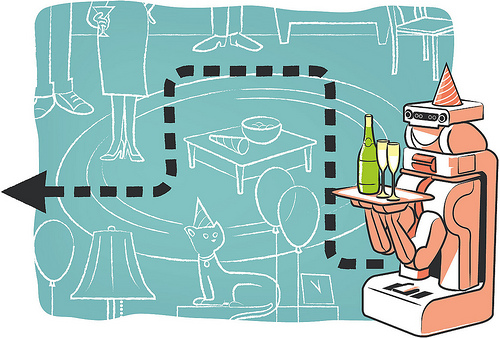
\includegraphics[width=.6\linewidth]{figure/task_path_planning}
\end{figure}

\end{frame}

\begin{frame}{Phenomena in Describing Tasks}{Path-Planning}

\begin{block}{}
\begin{itemize}
\item Humans tend to describe task instructions by natural language.\footnotemark
\end{itemize}
\end{block}

\begin{figure}
	\centering
	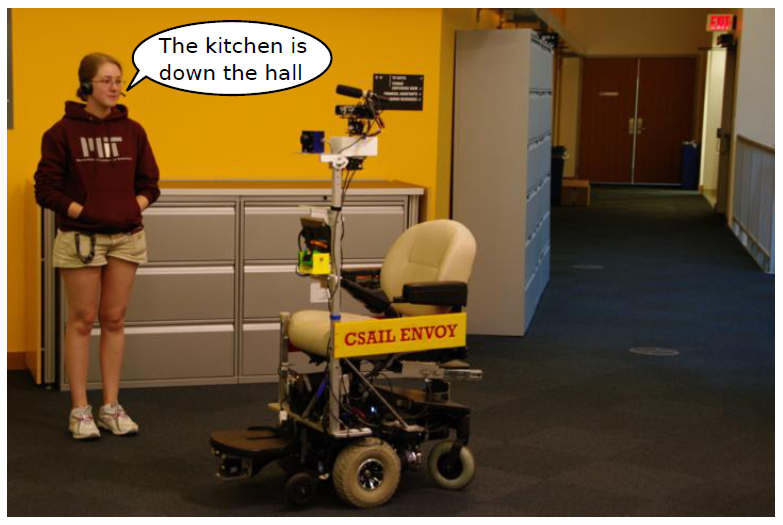
\includegraphics[width=.6\linewidth]{figure/natural_language}
	\caption{ \tiny{ Walter et al. "Learning semantic maps from natural language descriptions." {\it Robotics: Science and Systems, 2013}.} }
\end{figure}

\footnotetext[1]{\tiny {\it Kollar et al.} ``Toward understanding natural language directions.'' , 5th ACM/IEEE International Conference on Human-Robot Interaction (HRI) 2010.}

\end{frame}

\begin{frame}{Phenomena in Describing Tasks}{Path-Planning}

\begin{block}{}
\begin{itemize}
\item There often exist multiple objectives in a human's instruction.\footnotemark
\end{itemize}
\end{block}

\begin{figure}
	\centering
	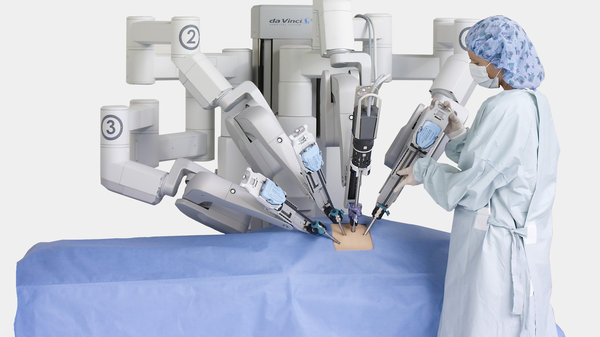
\includegraphics[width=.6\linewidth]{figure/surgery_robot}
	\caption{Tradeoff between distance and safety\footnotemark}
\end{figure}

\footnotetext[2]{\tiny {\it Rachmawati et al. } ``Preference incorporation in multi-objective evolutionary algorithms: A survey.'' , IEEE Congress on Evolutionary Computation (CEC) 2006.}

\footnotetext[3]{\tiny http://www.npr.org/sections/13.7/2013/05/16/184252284/facing-cancer-with-a-robot-surgeon-on-my-team}

\end{frame}

\begin{frame}{Phenomena in Describing Tasks}{Path-Planning}

\begin{block}{}
\begin{itemize}
\item Humans often have topological preferences for planned paths.\footnotemark
\end{itemize}
\end{block}

\begin{figure}
	\centering
	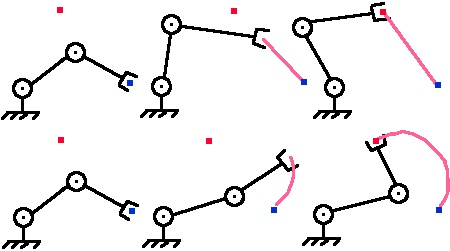
\includegraphics[width=.5\linewidth]{figure/robot_arm_path}
	\caption{\tiny http://www.societyofrobots.com/robot\_arm\_tutorial.shtml}
\end{figure}

\footnotetext[4]{\tiny {\it Bhattacharya et al.} ``Topological constraints in search-based robot path planning.'' Autonomous Robots 2012.}

\end{frame}

\begin{frame}{Problems}{Path-Planning}

\begin{block}{}
How to understand a human's command?
\end{block}

\begin{block}{}
How to deal with the ambiguity in the human's command?
\end{block}

\end{frame}


